\appendix
\addcontentsline{toc}{part}{Annexe}
%\markboth{\textbf{Annexe}}{}
\thispagestyle{empty}
\chapter{Les modèles IRT en code Stan.}


\begin{lstlisting}[language=Stan,caption={Code Stan pour le modèle de Rasch},basicstyle=\scriptsize, frame=lines,framesep=4.5mm,framexleftmargin=2.5mm,tabsize=2,numbers=left,fillcolor=\color{white},rulecolor=\color{black},numberstyle=\normalfont\scriptsize\color{black}]
    _1pl_model = """
    data {
        // numbers of things
        int<lower=1> N;  // number of observations
        int<lower=1> I;  // items,  number of questions  
        int<lower=1> S;  // subjects,  number of users 
        // data
        int<lower=1,upper=I> item[N];
        int<lower=1,upper=S> subject[N];
        int<lower=0,upper=1> grade[N];
        // data for posterior prediction using new data also used for Cross-validation
        int<lower=1> N_new;
        int<lower=1,upper=I> item_new[N_new];
        int<lower=1,upper=S> subject_new[N_new];
    }
    parameters {
        // parameters
        real ability[S];             //  alpha: ability of student
        real difficulty[I];          //  beta: difficulty of question
        real delta;                   // mean student ability
    }
    model {
        ability ~ normal(0,1);         
        difficulty ~ normal(0,1);   
        delta ~ normal(0.75,1);
        for(n in 1:N)
            grade[n] ~ bernoulli_logit(ability[subject[n]] - difficulty[item[n]] + delta);
    }
    generated quantities {
        int<lower=0,upper=1> y_pred[N];
        int<lower=0,upper=1> yNew_pred[N_new];
        vector[N] log_lik;

        for(n in 1:N){
            y_pred[n] = bernoulli_logit_rng(ability[subject[n]] - difficulty[item[n]] + delta);
            log_lik[n] = bernoulli_logit_lpmf( grade[n] | ability[subject[n]] - difficulty[item[n]]
            + delta);
        }
        for (n in 1:N_new) {
            yNew_pred[n] = bernoulli_logit_rng(ability[subject_new[n]] - difficulty[item_new[n]] + delta);                                             
        }
    }
    """
\end{lstlisting}
\newpage

\begin{lstlisting}[language=Stan,caption={Code Stan pour 2PL},basicstyle=\scriptsize, frame=lines,framesep=4.5mm,framexleftmargin=2.5mm,tabsize=2,numbers=left,fillcolor=\color{white},rulecolor=\color{black},numberstyle=\normalfont\scriptsize\color{black}]
    _2pl_model = """
    data {
        // numbers of things
        int<lower=1> N;  // number of observations
        int<lower=1> I;  // items,  number of questions  
        int<lower=1> S;  // subjects,  number of users 
        // data
        int<lower=1,upper=I> item[N];
        int<lower=1,upper=S> subject[N];
        int<lower=0,upper=1> grade[N];
        // data for posterior prediction using new data also used for Cross-validation
        int<lower=1> N_new;
        int<lower=1,upper=I> item_new[N_new];
        int<lower=1,upper=S> subject_new[N_new];
    }
    parameters {
        // parameters
        real ability[S];             //  alpha: ability of student
        real difficulty[I];          //  beta: difficulty of question
        vector<lower=0>[I] discrimination;      // discrimination of question
        real delta;                   // mean student ability
    }
    model {
        ability ~ normal(0,1);         
        difficulty ~ normal(0,1);   
        discrimination ~ lognormal(0,1);
        delta ~ normal(0.75,1);
        grade ~ bernoulli_logit(discrimination[item] .* (ability[subject] - (difficulty[item] + delta)));	
    }
    generated quantities {
        int<lower=0,upper=1> y_pred[N];
        int<lower=0,upper=1> yNew_pred[N_new];
        vector[N] log_lik;

        for(n in 1:N){
            y_pred[n] = bernoulli_logit_rng(discrimination[item[n]] * (ability[subject[n]] - (difficulty[item[n]] + delta)));
            log_lik[n] = bernoulli_logit_lpmf( grade[n] | discrimination[item[n]] * (ability[subject[n]] - (difficulty[item[n]] + delta)));
        }
        for (n in 1:N_new) {
            yNew_pred[n] = bernoulli_logit_rng(discrimination[item[n]] * (ability[subject_new[n]] - (difficulty[item_new[n]] + delta)));                             
        }
    }
    """
\end{lstlisting}

\newpage

\begin{lstlisting}[language=Stan,caption={Code Stan pour 3PL},basicstyle=\scriptsize, frame=lines,framesep=4.5mm,framexleftmargin=2.5mm,tabsize=2,numbers=left,fillcolor=\color{white},rulecolor=\color{black},numberstyle=\normalfont\scriptsize\color{black}]
    _3pl_model = """
    data {
        // numbers of things
        int<lower=1> N;  // number of observations
        int<lower=1> I;  // items,  number of questions  
        int<lower=1> S;  // subjects,  number of users 
        // data
        int<lower=1,upper=I> item[N];
        int<lower=1,upper=S> subject[N];
        int<lower=0,upper=1> grade[N];
        // data for posterior prediction using new data also used for Cross-validation
        int<lower=1> N_new;
        int<lower=1,upper=I> item_new[N_new];
        int<lower=1,upper=S> subject_new[N_new];
    }
    parameters {
        // parameters
        real ability[S];             //  alpha: ability of student
        real difficulty[I];          //  beta: difficulty of question
        vector<lower=0>[I] discrimination;      // discrimination of question
        vector<lower=0,upper=1>[I] guessing;    
        real delta;                   // mean student ability
    }
    model {
        ability ~ normal(0,1);         
        difficulty ~ normal(0,1);   
        discrimination ~ lognormal(0,1);
        guessing ~ beta(5,17);
        delta ~ normal(0.75,1);
        grade ~ bernoulli(guessing[item] + ((1-guessing[item]).*(inv_logit(discrimination[item] .* (ability[subject] - (difficulty[item] + delta))))));
    }
    generated quantities {
        int<lower=0,upper=1> y_pred[N];
        int<lower=0,upper=1> yNew_pred[N_new];
        vector[N] log_lik;

        for(n in 1:N){
            y_pred[n] = bernoulli_rng(guessing[item[n]] + ((1-guessing[item[n]]) * (inv_logit(discrimination[item[n]] .* (ability[subject[n]] - (difficulty[item[n]] + delta))))));
            log_lik[n] = bernoulli_lpmf( grade[n] | guessing[item[n]] + ((1-guessing[item[n]]) * (inv_logit(discrimination[item[n]] .* (ability[subject[n]] - (difficulty[item[n]] + delta))))));
        }
        for (n in 1:N_new) {
            yNew_pred[n] = bernoulli_rng(guessing[item[n]] + ((1-guessing[item[n]]) * (inv_logit(discrimination[item[n]] .* (ability[subject[n]] - (difficulty[item[n]] + delta))))));                                             
        }
    }
    """
\end{lstlisting}

\begin{lstlisting}[language=Stan,caption={Code Stan pour le modèle de Rasch avec cross-validation},basicstyle=\scriptsize, frame=lines,framesep=4.5mm,framexleftmargin=2.5mm,tabsize=2,numbers=left,fillcolor=\color{white},rulecolor=\color{black},numberstyle=\normalfont\scriptsize\color{black}]
    _1pl_cross_val_model = """
    functions {
        int[] permutation_rng(int N) {
            int y[N];
            for (n in 1:N)
                y[n] = n;
            vector[N] theta = rep_vector(1.0 / N, N);
            for (n in 1:N){
                int i = categorical_rng(theta);
                int temp = y[n];
                y[n] = y[i];
                y[i] = temp;
            }
            return y;
        }
    }
    
    data {
      // numbers of things
      
      int<lower=1> N;  // number of observations
      int<lower = 0, upper = N> N_test;
      int<lower=1> I;  // items,  number of questions  
      int<lower=1> S;  // subjects,  number of users
      
      // data
      
      int<lower=1,upper=I> item[N];
      int<lower=1,upper=S> subject[N];
      int<lower=0,upper=1> grade[N];
    }
    transformed data {
      int N_train = N - N_test;
      int permutation[N] = permutation_rng(N);
      // train
      int item_train[N_train] = item[permutation[1 : N_train]];
      int subject_train[N_train]  = subject[permutation[1 : N_train]];
      int grade_train[N_train]  = grade[permutation[1 : N_train]];
      int s_train = size(subject_train);
      int i_train = size(item_train);
      
      
      // test
      int item_test[N_test] = item[permutation[N_train + 1 : N]];
      int subject_test[N_test] = subject[permutation[N_train + 1 : N]];
      int grade_test[N_test] = grade[permutation[N_train + 1 : N]];
    }
    parameters {
      // parameters
      real ability[s_train];             //  alpha: ability od student
      real difficulty[i_train];          //  beta: difficulty of question
      real delta;                   // man student ability
      
    }
    model {
    
      ability ~ normal(0,1);         
      difficulty ~ normal(0,1);   
      delta ~ normal(0.75,1);
      
      for (n in 1:N_train) {
          grade_train[n] ~ bernoulli_logit(ability[subject_train[n]] - difficulty[item_train[n]] + delta);
      }
      
    }
    generated quantities {
      int<lower=0,upper=1> grade_pred[N_test];
      int<lower=0,upper=1> grade_observed[N_test];
      grade_observed = grade_test;
      
      for (n in 1:N_test) {
        grade_pred[n] = bernoulli_logit_rng(ability[subject_test[n]] - difficulty[item_test[n]] + delta);
      }
    }
    """
\end{lstlisting}

\chapter{Les distributions des modèles.}
\begin{figure}[H]
	\begin{center}
		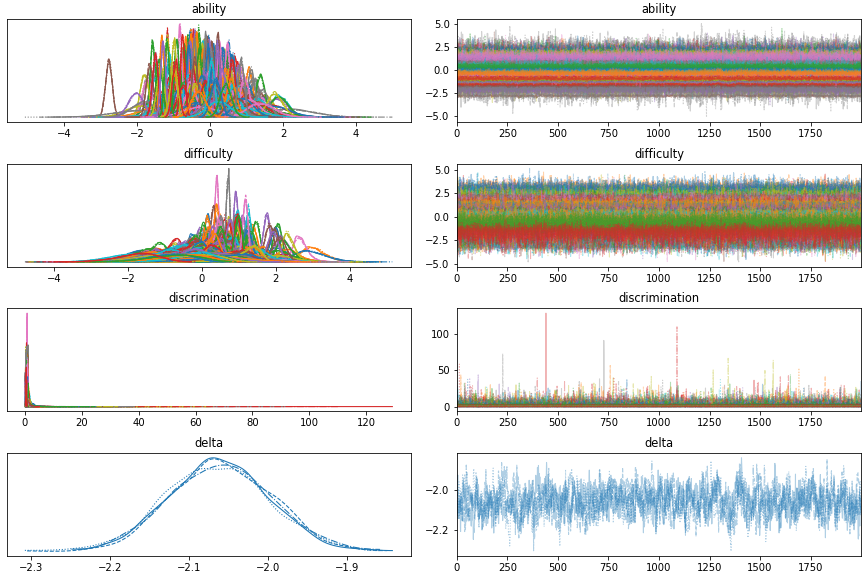
\includegraphics[width=\textwidth]{images/annexe/model_plot-trace2.png}
	\end{center}
	\caption{Les distributions postérieures du modèle logistique à deux paramètres.}
	\label{model_trace-plot2}
\end{figure}

\begin{figure}[H]
	\begin{center}
		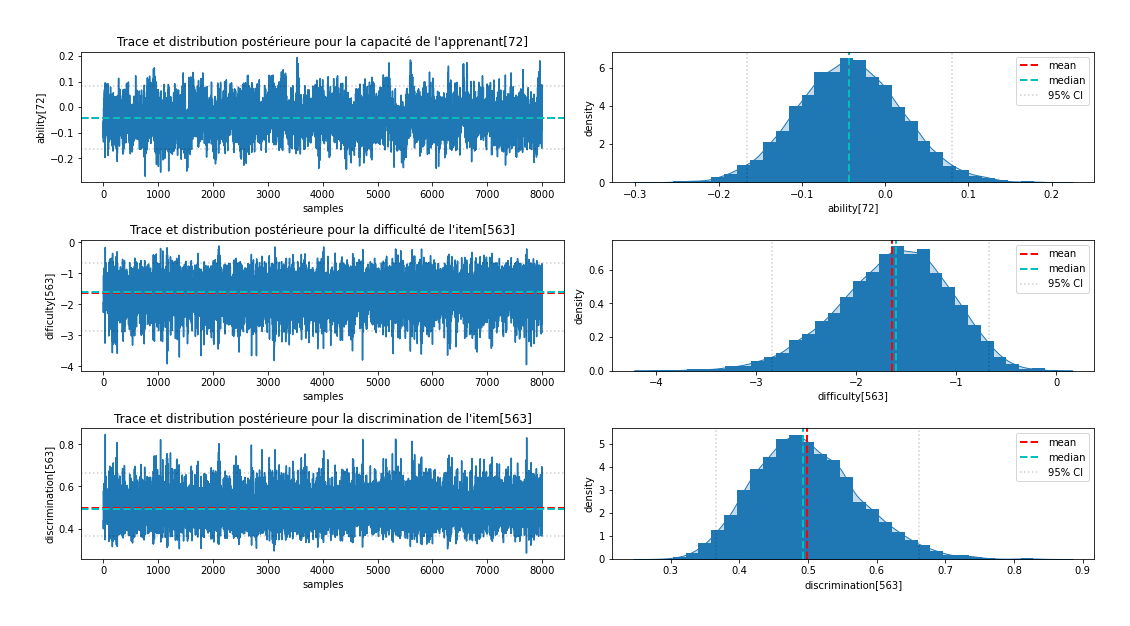
\includegraphics[width=\textwidth]{images/annexe/params_posterior_distribution2.png}
	\end{center}
	\caption{Distribution postérieure de la capacité de l’apprenant[72], de la difficulté de l’item[563] et de la discrimination de l’item[563] du modèle 2PL.}
	\label{params_posterior_distribution_2pl}
\end{figure}

\begin{figure}[H]
	\begin{center}
		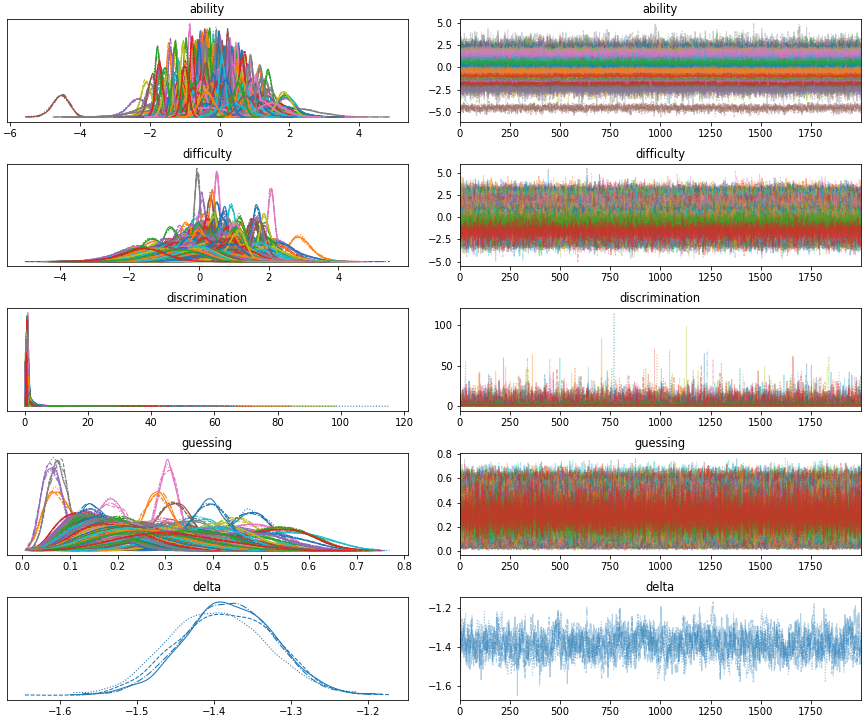
\includegraphics[width=\textwidth]{images/annexe/model_plot-trace3.png}
	\end{center}
	\caption{Les distributions postérieures du modèle logistique à trois paramètres.}
	\label{model_trace-plot3}
\end{figure}

\begin{figure}[H]
	\begin{center}
		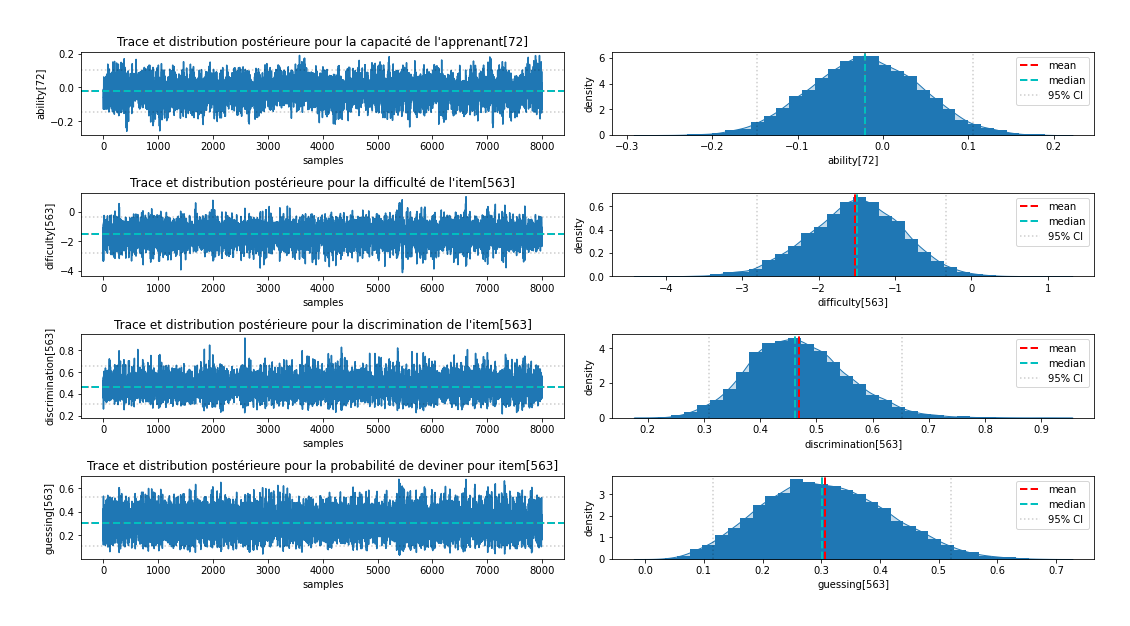
\includegraphics[width=\textwidth]{images/annexe/params_posterior_distribution3.png}
	\end{center}
	\caption{Distribution postérieure de la capacité de l’apprenant[72], de la difficulté de l’item[563], de la discrimination de l’item[563] et de la chance de deviner la reponse correcte de l'item[563] du modèle 2PL.}
	\label{params_posterior_distribution_3pl}
\end{figure}